\documentclass[crop,tikz]{standalone}
\usepackage{tikz}
\usetikzlibrary{matrix,backgrounds,arrows.meta,fit,positioning}
\begin{document}

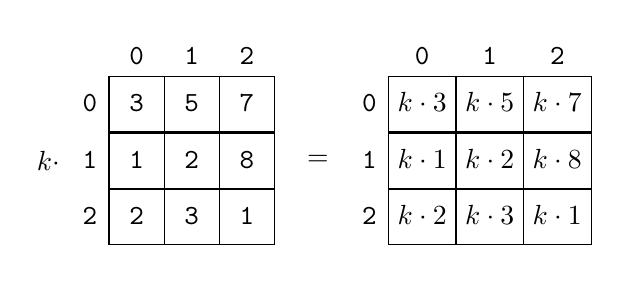
\begin{tikzpicture}[font=\ttfamily,
  array/.style={matrix of nodes,nodes={draw, minimum size=7mm},column sep=-\pgflinewidth, row sep=0mm, nodes in empty cells,text height=1.5ex, text depth=.25ex,
    row 1/.style={nodes={draw=none, fill=none, minimum size=5mm}},
    column 1/.style={nodes={draw=none, fill=none, minimum size=5mm}},
}]

\matrix[array] (matrix) {
  & 0 & 1 & 2 \\
0 & 3 & 5 & 7 \\
1 & 1 & 2 & 8 \\
2 & 2 & 3 & 1 \\ };

\node[left=0cm of matrix-3-1.west] {$k \cdot $};
\node[right=1cm of matrix-3-4.west] {$=$};

\matrix[array,right=0.7cm of matrix] (result) {
  & 0 & 1 & 2 \\
0 & $k \cdot 3 $ & $k \cdot 5 $ & $k \cdot 7 $ \\
1 & $k \cdot 1 $ & $k \cdot 2 $ & $k \cdot 8 $ \\
2 & $k \cdot 2 $ & $k \cdot 3 $ & $k \cdot 1 $ \\
};

\end{tikzpicture}
\end{document}
